\subsubsection{curve-assert-valid}
\label{curve-assert-valid}

Take curve-secp256k1 as example, the same as other texs.

\begin{enumerate}
    \item target
        check point is on the curve, y\^2 = x\^3 + ax +b
    \item curve-assert-valid process layout
        \begin{figure}[!ht]
            \centering
            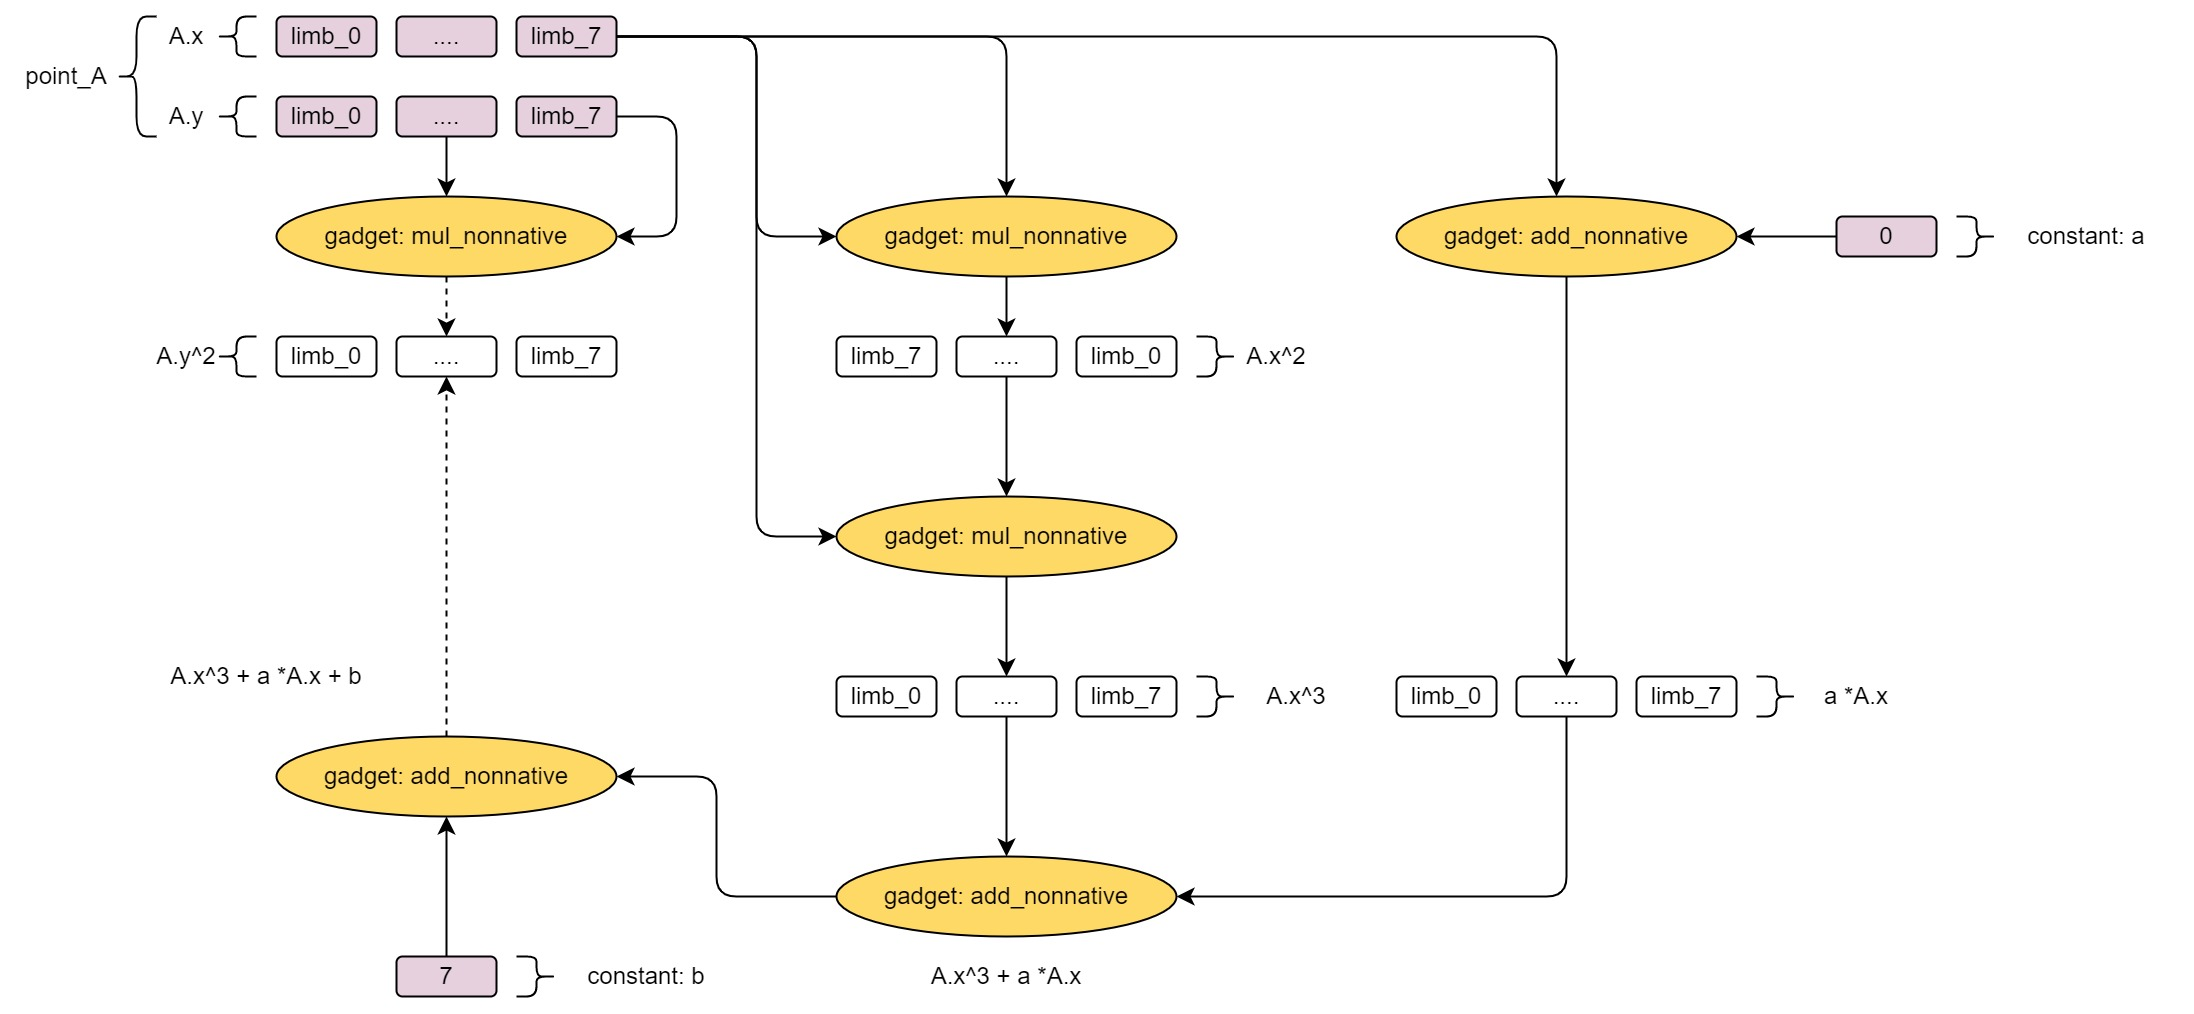
\includegraphics[width=0.8\textwidth]{curve-assert-valid-layout.jpg}
            \caption{curve-assert valid layout}
            \label{fig:curve-assert-valid-layout}
        \end{figure}
    \item constraints-info and costs
        \begin{itemize}
            \item gadget-add-nonnative num: 3
            \item gadget-mul-nonnative num: 3
            \item gate type num: 13
                \begin{itemize}
                    \item 8: U32AddManyGate{2,3,5,7,9,11,13,15}
                    \item 1: ComparisonGate
                    \item 1: ArithmeticGate
                    \item 1: U32ArithmeticGate
                    \item 2: U32RangeCheckGate{0,8}
                \end{itemize}
        \end{itemize}

\end{enumerate}